
\documentclass{article}

\usepackage[margin=1in]{geometry} 
\usepackage{graphicx, amsmath, amsthm, amssymb, mathds, centernot}
\usepackage{physics, braket}
\newcommand*\dif{\mathrm{d}}
\newcommand*\ee{\mathrm{e}}
\newcommand*\ii{\mathds{1}}
\newcommand*{\fsl}[1]{\centernot{#1}}

\begin{document}
\title{Charged Black Holes: Why We May Ignore Them}
\author{Randy Kayser\\ General Relativity final}

\maketitle

\section{Determining the Metric of a Charged Black Hole}
We seek a static, spherically symmetric solution to the EFEs in the presence of an electromagnetic field $A_{\mu} = (-f(r), 0,0,0)$. Knowing that if $A_{\mu} = 0$, our result should reproduce the Schwartzschild metric, guess a metric of the following form:

\begin{equation*}
   \dif s^2 = -(1+h(r))\dif t^2 + (1 + h(r))^{-1}\dif r^2 + r^2 \dif \Omega^2
\end{equation*}

The maxwell tensor is given by:

\begin{equation*}
   F_{\mu\nu} = 2\nabla_{[\mu}A_{\nu]} = 2\partial_{[\mu}A_{\nu]} \\
\end{equation*}
Whose only nonvanishing components are:
\begin{equation*}
   F_{tr} = -F_{rt} = -F^{tr} = F^{rt} = \partial_r f(r)
\end{equation*}
The Stress-Energy tensor of the Electromagnetic Field is given by:
\begin{equation*}
   T_{\mu\nu} = F_{\mu}^{\hspace{5px}\alpha}F_{\nu\alpha} - \frac{1}{4}F_{\alpha\beta}F^{\alpha\beta}
\end{equation*}
The non-zero $(1,1)$ components of this tensor are given by:
\begin{align*}
   T^t_{\hspace{5px}t} &= -\frac{1}{2}\partial_rf(r) \\
   T^r_{\hspace{5px}r} &= -\frac{1}{2}\partial_rf(r) \\
   T^{\theta}_{\hspace{5px}\theta} &= \frac{1}{2}\partial_rf(r) \\
   T^{\phi}_{\hspace{5px}\phi} &= \frac{1}{2}\partial_rf(r) \\
   \implies T^{\mu}_{\hspace{5px}\mu} &= 0 \\
   \implies G^{\mu}_{\hspace{5px}\mu} &= 0 \\
\end{align*}
Where the last implication is satisfied due to the EFEs.
Computing the non-zero Christoffel symbols yields:
\begin{align*}
   \Gamma^{t}_{rt} &= \frac{1}{2}\frac{h'(r)}{1+h(r)} \\
   \Gamma^{r}_{tt} &= \frac{1}{2}(1+h(r))h'(r) \\
   \Gamma^{r}_{rr} &= -\frac{1}{2}\frac{h'(r)}{1+h(r)} \\
   \Gamma^{r}_{\theta\theta} &= -r(1+h(r)) \\
   \Gamma^r_{\phi\phi} &= -r(1+h(r))\sin^2\theta \\
   \Gamma^{\theta}_{\theta r} &= \frac{1}{r} \\
   \Gamma^{\theta}_{\phi\phi} &= -\cos\theta\sin\theta \\
   \Gamma^{\phi}_{\phi\theta} &= \cot\theta \\
\end{align*}
Thus, the (non-zero) components of the Ricci Tensor and the Ricci scalar are given by:
\begin{align*}
   R_{tt} &= \frac{(1+h(r))(2h'(r) + rh' '(r))}{2r} \\
   R_{rr} &= \frac{h'(r) + rh' '(r)}{2r(1+h(r))} \\
   R_{\theta\theta} &= -h'(r) - rh' '(r) \\
   R_{\phi\phi} &= -\sin^2\theta(h(r) + rh'(r)) \\
   R &= -\frac{2h(r) + 4rh'(r) + r^2h' '(r)}{r^2} \\
\end{align*}

Computing the trace of the resulting einstein tensor yields:
\begin{equation*}
   \frac{2h(r) + 4rh'(r)+r^2h''(r)}{r^2} = 0
\end{equation*}

Guess a solution of the form $h(r) = r^{\alpha}$. Then, obtain:
\begin{align*}
   2r^{\alpha - 2} + r\alpha r^{\alpha - 2} + \alpha(\alpha - 1)r^{\alpha - 2} &= 0 \\
   \implies \alpha^2 + 3\alpha + 2 &= 0 \\
   \implies \alpha &= -1, -2 \\
\end{align*}
Thus, $h(r) = \frac{A}{r} + \frac{B}{r^2}$. Now, use the $3,3$ component of the EFEs to determine $f(r)$.
\begin{align*}
   \frac{1}{2} r\big(2h'(r) + rh' '(r)\big) &= 4\pi r^2 \big(f'(r)\big)^2 \\
   \implies f(r) &= \sqrt{\frac{B}{4\pi}}\frac{1}{r^2} \\
\end{align*}
Identifying the resulting stress energy tensor with that of a point charge $Q$ located at the origin fixes $B = Q^2$ in gaussian units.
\section{Killing Vectors and the Geodesic Equation}
Because of spherical symmetry, all orbits are contained in a plane. Thus, without loss of generality, set $\theta = \frac{\pi}{2}$. Then, the metric becomes:
\begin{equation*}
   \dif s^2 = -\big(1 - \frac{2M}{r} + \frac{Q^2}{r^2}\big)\dif t^2 + \frac{\dif r^2}{1 - \frac{2M}{r} + \frac{Q^2}{r^2}} + r^2\dif \theta^2
\end{equation*}
This metric admits two killing fields, $(1,0,0,0)$ and $(0,0,1,0)$, thus, along a geodesic, $p^0 = E$ and $p^{\theta} = l$ are conserved. Because this space is asymptotically flat, we can relate these quantities as the Energy and Angular Momentum at infinity. Computing the norm of the 4-momentum, obtain:
\begin{align*}
   0 &= -\frac{E^2}{1 - \frac{2M}{r} + \frac{Q^2}{r^2}} + \frac{1}{1 - \frac{2M}{r} + \frac{Q^2}{r^2}}\big(\frac{\dif r}{\dif \lambda}\big)^2 + \frac{L^2}{r^2} + m^2 \\
   \implies \frac{\dif r}{\dif \tau} &= \pm \sqrt{|\tilde{E}^2 - V^2|} \\
   V^2 &= \big(1 - \frac{2M}{r} + \frac{Q^2}{r^2}\big)\big(1 + \frac{\tilde{l}^2}{r^2}\big)
\end{align*}
Where $\lambda$ is an affine parameter of the geodesic, and $\tilde{E}$ and $\tilde{l}$ represent the energy and angular momentum per unit rest mass. V is the effective potential, analogous to the uncharged case. 
\section{Numerically Integrating the Resulting Geodesic Equation}
Figure 1 shows the proper time for the radial plunge of a neutral test particle from $r = 20 r_s$ as a function of $Q/M$. Times have been normalized so that the proper time of the plunge for an uncharged black hole is unity. Note the sharp dependence on $Q/M$, and that the maximum possible value attainable is $\approx 1.35$. Thus, due to bounds that can be placed on $Q/M$ (below), we establish that the charge of a black hole cannot significantly contribute to the dynamics of a neutral test particle.

\begin{figure}
   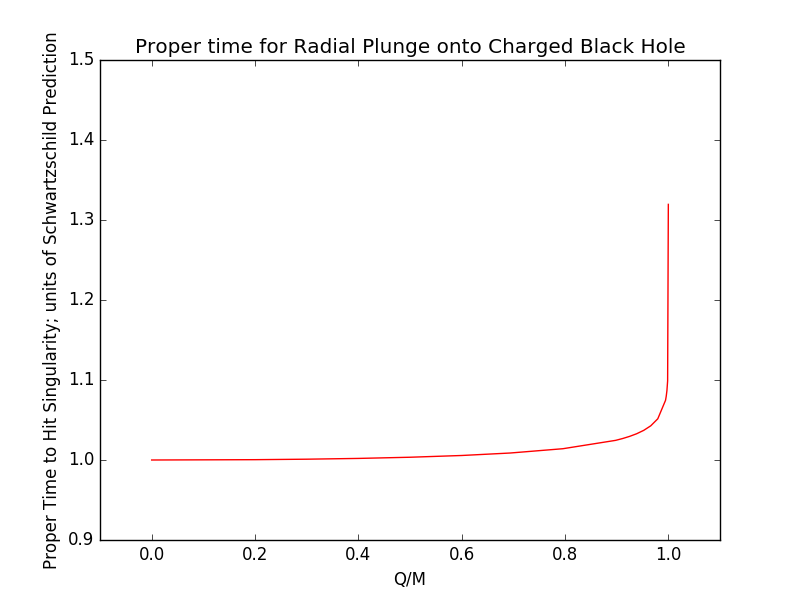
\includegraphics[width=8cm]{Schwartzschild_Comparison.png}
\end{figure}

\section{Bounds on Q/M}
The Reissner-Nordstrom metric contains two event horizons, where $g_{rr}$ diverges.
setting the denominator to zero, obtain:
\begin{align*}
   r^2 - 2Mr + Q^2 &= 0 \\
   \implies r_{\pm} &= M \pm \sqrt{MQ - Q^2}
\end{align*}
If $Q > M$, then this result is unphysical, as it results in a naked singularly. Thus, we have shown a surpising result: A black hole cannot have more charge than mass, in natural units. Such a system cannot gravitationally collapse.
\vspace{10pt} Code:
\begin{verbatim}
   http://github.com/RandallKayser/GR_Final
\end{verbatim}
\end{document}

